\documentclass[conference,a4paper]{IEEEtran}
\usepackage[T1]{fontenc}
\usepackage{cite}
\usepackage{amsmath,amssymb}
\usepackage{graphicx}
\usepackage{booktabs}
\usepackage{url}
\urlstyle{same}
\usepackage[hidelinks]{hyperref}
\hypersetup{pdftitle={InsightPulse: Contextual Sentiment Analysis and Aspect-Level Insights from Customer Feedback},pdfauthor={Monil Patel},pdfsubject={Fifth-semester Artificial Intelligence project report}}
\hyphenation{Insight-Pulse}
\begin{document}
\title{InsightPulse: Contextual Sentiment Analysis and\mbox{ Aspect-Level Insights} from Customer Feedback}
\author{\IEEEauthorblockN{Monil Patel}
\IEEEauthorblockA{Department of Computer Science and Engineering\\Jain University, India}}
\maketitle

\begin{abstract}
Customer feedback spreadsheets contain valuable opinions, but inconsistent file structures and context-dependent language complicate reliable analysis. This paper presents InsightPulse, a local web application for English sentiment classification, aspect-level evidence extraction, and feedback exploration. The system combines a pretrained BERT product-review classifier with a locally trained, calibrated linear support vector machine using word and character term frequency--inverse document frequency features. A deterministic routing policy introduces specialist evidence for short factual statements, mild criticism, and uncertain contextual predictions. The ingestion layer supports CSV, TSV, and Excel files, provides explicit column mapping, preserves source rows, and reports invalid or uncertain entries. Five business aspects are identified through contextual lexical rules, while latent Dirichlet allocation supplies exploratory topic labels. On a fixed 594-review positive/negative development benchmark, the hybrid obtains 538 correct predictions (90.57\%), compared with 503 (84.68\%) for the local SVM. Three supplied files containing 1,349 rows were processed, and 30 regression tests passed. These findings demonstrate a functioning analysis workflow and improved development-benchmark performance; they do not establish independent three-class or target-domain accuracy. Benchmark reuse, unknown pretrained-data overlap, and limited neutral-label coverage remain explicit limitations.
\end{abstract}
\begin{IEEEkeywords}
sentiment analysis, BERT, support vector machine, customer feedback, aspect analysis, spreadsheet ingestion
\end{IEEEkeywords}

\section{Introduction}
Organizations receive feedback through product reviews, support forms, and survey spreadsheets. A sentiment label can summarize whether a customer is satisfied, but an actionable interpretation also requires identifying the issue being discussed. A positive opinion about product quality may coexist with a complaint about delivery. Moreover, an analysis pipeline can produce misleading totals if it selects a customer-name column, ignores blank records, or treats a report title as the table header.

InsightPulse addresses these practical problems as an academic artificial intelligence project. Its objective is to make English customer feedback easier to inspect while retaining the original evidence. Users can analyze one review or upload a tabular file, choose the feedback column, examine sentiment and business-aspect summaries, and export every input row with its analysis status. The application operates locally and requires no external inference API.

The implementation integrates established methods rather than proposing a new language-model architecture. Its contributions are: (1) a shared contextual and classical sentiment pipeline for single and batch analysis; (2) an ingestion workflow with preview, header detection, explicit column selection, and row accountability; (3) contextual aspect rules that distinguish product use from seller logistics; and (4) reproducible evaluation that separates development-benchmark results from unsupported claims about future customer data. The distinction is essential because confidence scores, sentiment proportions, and classification accuracy answer different questions.

\section{Related Work}
Classical sentiment classification uses labeled examples to associate text features with opinion polarity. Pang, Lee, and Vaithyanathan compared machine-learning techniques for sentiment classification, establishing a useful starting point for statistical review analysis~\cite{pang}. InsightPulse retains this approach through four classical candidates and explicit cross-validation. The scikit-learn framework supplies consistent interfaces for feature extraction, model fitting, calibration, and evaluation~\cite{sklearn}.

BERT learns contextual text representations using a Transformer encoder that conditions on surrounding words~\cite{bert}. Contextual representations are relevant when a review describes a problem that the product successfully solves: negative words alone need not imply a negative product opinion. InsightPulse uses NLP Town's released multilingual BERT checkpoint, which was fine-tuned by its provider to predict one to five stars from product reviews~\cite{nlptown}. The present project performs inference with this checkpoint; it does not claim to have pretrained or fine-tuned BERT. Although the underlying checkpoint supports several languages, the application's supported scope is English.

Topic discovery complements sentiment classification by exposing groups of co-occurring terms. Latent Dirichlet allocation (LDA) represents documents through mixtures of latent topics~\cite{lda}. Here, LDA provides exploratory labels learned from the local training corpus. Business aspects are handled separately through a predefined vocabulary and contextual rules; an LDA topic is not treated as an independently verified business category.

The UCI Sentiment Labelled Sentences dataset supplies positive and negative examples drawn from Amazon, Yelp, and IMDb~\cite{uci}. Its deliberately binary labels make it useful for polarity checks but insufficient for measuring neutral-class performance. This paper uses that distinction throughout its evaluation.

\section{System Design and Implementation}
\subsection{Architecture}
The application separates presentation, ingestion, inference, and aggregation. Figure~\ref{fig:architecture} summarizes the implemented flow. Python 3.12 and Flask expose prediction and file-upload endpoints. The browser interface uses HTML, CSS, and JavaScript, with asynchronous requests to the local server. pandas represents tabular data, openpyxl reads Excel workbooks, NumPy supports probability calculations, and joblib loads classical model artifacts. BERT executes through ONNX Runtime on the CPU.

\begin{figure}[t]
\centering
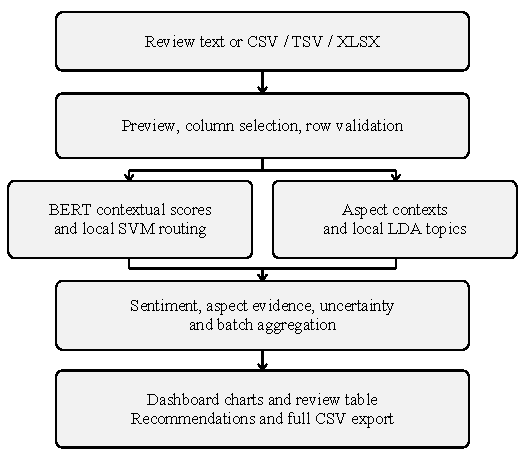
\includegraphics[width=\columnwidth]{architecture.pdf}
\caption{InsightPulse processing architecture. The sentiment service is reused for complete reviews and extracted aspect contexts.}
\label{fig:architecture}
\end{figure}

The dashboard has four views: review analysis, batch insights, model evaluation, and an explanation of the processing stages. Batch results show sentiment counts, aspect mentions, uncertainty flags, recommendations, and a searchable table. Pagination displays 25 records per page, while export includes the complete batch. Theme preferences are stored in the browser. No application database or user-account system is implemented; model files persist on disk, while uploaded data and inference results are handled in memory during processing.

\subsection{Application Interfaces}
The Flask interface provides \texttt{/api/predict} for a single review, \texttt{/api/preview\_upload} for file inspection, and \texttt{/api/batch\_upload} for analysis. The metrics endpoint exposes saved evaluation data and the active engine name. A separate endpoint supplies a sample dataset. JSON carries predictions and aggregates to the browser, where JavaScript renders the charts and tables. The same prediction module serves both single-review and batch requests, reducing discrepancies between the two workflows.

\subsection{Input and Export Controls}
Supported uploads are CSV, TSV, and \texttt{.xlsx} files, limited to 16~MB and 10,000 rows. Individual feedback entries are limited to 10,000 characters. CSV decoding attempts UTF-8, UTF-16, and Windows-1252; delimiter detection supports commas, tabs, semicolons, and pipes. Excel preview scans worksheets for recognizable feedback headers. Users can select another worksheet or column before analysis.

Header detection examines the first 20 rows for aliases such as \texttt{Feedback}, \texttt{Comments}, and \texttt{Feedback / Comments}. Titles above an identified header are reported and ignored. If selection is ambiguous, the application requires an explicit choice. Known metadata columns, including ratings, names, identifiers, and department labels, are excluded from automatic feedback selection. Duplicate normalized headers are rejected before pandas can silently rename them.

Blank and invalid entries remain visible as skipped rows. Repeated header rows embedded in a table are also skipped. Original columns are retained; collisions with generated column names are resolved by renaming the original field. Source-row indices help locate the corresponding record in the input table. For CSV fields containing embedded newlines, these indices represent logical records rather than physical text-line numbers. Spreadsheet exports escape formula-like cell prefixes so customer text is retained as literal data.

\section{Sentiment and Insight Methodology}
\subsection{Classical Representation and Training}
The local classifier uses deterministic preprocessing implemented with NLTK's offline Snowball stemmer. Contractions are expanded, formatting is removed, and negation and context words are retained for sentiment classification. This preprocessing path differs from the BERT path, which preserves punctuation and word order and does not stem its input.

Word unigrams, bigrams, and trigrams capture terms and short phrases. Character sequences of length three to five supply evidence for spelling variations. The two TF-IDF feature blocks are combined as
\begin{equation}
\mathbf{x}(d)=[\mathbf{x}_{w}(d);\;0.45\mathbf{x}_{c}(d)],
\end{equation}
where $d$ is a review. The word and character vocabularies are limited to 18,000 and 14,000 features, respectively. With sublinear term frequency and smoothed inverse document frequency, a nonzero feature weight before vector normalization is
\begin{equation}
w_{t,d}=(1+\log f_{t,d})\left[\log\frac{1+N}{1+\operatorname{df}(t)}+1\right].
\end{equation}
Here, $f_{t,d}$ is the term count, $N$ is the number of fitting documents, and $\operatorname{df}(t)$ is document frequency. Absent terms have zero weight.

The candidates are multinomial Naive Bayes, logistic regression, calibrated linear SVM, and random forest. The random forest contains 80 trees with maximum depth 32. Logistic regression and SVM use balanced class weights. The SVM uses $C=1$ with three-fold probability calibration. Candidate selection uses five-fold stratified cross-validation and the highest training macro-F1; TF-IDF is fitted inside each outer fold. The selected classifier and feature transformer are saved separately.

\subsection{Contextual BERT Inference}
The active contextual model is NLP Town's multilingual uncased BERT classifier for product-review sentiment~\cite{nlptown}. A pinned Xenova ONNX conversion is used for reproducibility~\cite{xenova}. Quantization reduces numerical precision for inference; it is an execution optimization and does not itself establish improved accuracy~\cite{onnx}. The provider's model is used as released, without additional gradient-based training in this project.

Let $p_k$ denote the predicted probability of star rating $k$. Three sentiment scores are obtained by summing the relevant classes:
\begin{align}
p_B(\mathrm{Negative}) &= p_1+p_2,\\
p_B(\mathrm{Neutral}) &= p_3,\\
p_B(\mathrm{Positive}) &= p_4+p_5.
\end{align}
This mapping assumes that three-star opinions are a useful proxy for neutral feedback. It does not make star ratings and semantic neutrality identical. Consequently, short factual statements receive additional treatment in the hybrid policy.

The tokenizer processes windows of at most 512 tokens with a 64-token overlap. All windows contribute to the document score, using weights based on newly covered tokens. A disagreement between positive and negative window labels triggers review. Common positive idioms, such as ``not bad at all,'' are normalized by explicit rules before tokenization, while the original review is retained for display and export. These rules are development heuristics and may fail on unusual constructions.

Each window is inferred separately to avoid a review's prediction changing with neighboring examples under dynamic quantization. A bounded cache stores up to 2,048 normalized text results in memory. Repeated reviews therefore reduce computation, but duplicates are still retained in the reported batch totals.

\subsection{Hybrid Routing and Uncertainty}
Let $p_S$ be the calibrated local SVM distribution and $p_B$ the mapped BERT distribution. The final distribution is
\begin{equation}
p(y\mid d)=\alpha(d)p_S(y\mid d)+(1-\alpha(d))p_B(y\mid d).
\label{eq:hybrid}
\end{equation}
Table~\ref{tab:routing} specifies the ordered rules used to choose $\alpha$. Only the first matching rule is applied. The routing policy is manually specified; it is not a learned gating network. The final class is the maximum-score class from (\ref{eq:hybrid}).

\begin{table}[t]
\caption{Ordered Hybrid Routing Policy}
\label{tab:routing}
\centering\footnotesize
\begin{tabular}{p{0.77\columnwidth}r}
\toprule
First matching condition & $\alpha$\\\midrule
At most 20 words; SVM neutral score $\geq0.75$; maximum BERT score $<0.80$ & 0.75\\
Recognized mild-criticism phrase; SVM negative score $\geq0.80$; maximum BERT score $<0.80$ & 0.60\\
Maximum BERT score $<0.60$ and maximum SVM score $\geq0.70$ & 0.65\\
Otherwise & 0.00\\\bottomrule
\end{tabular}
\end{table}

The mild-criticism rule recognizes phrases including ``could be better'' and ``needs improvement.'' A review is flagged when the maximum final score is below 0.60, the margin between its two highest scores is below 0.15, no known whole-word features are found, positive and negative windows disagree, or the uncertain-context fallback combines conflicting labels. An uncertain aspect prediction also flags the full review. Flags identify records for inspection; absence of a flag is not proof of correctness. Despite the calibrated SVM component, the final hybrid scores have not been calibrated against independent customer data.

\subsection{Aspect Evidence and Topics}
Aspect extraction matches normalized whole words and phrases against five business vocabularies: Product Quality, Customer Support, Delivery \& Packaging, Pricing \& Value, and Usability \& UI. Contextual guards suppress misleading matches. For example, tracking lost keys or locating airport luggage describes product functionality and should not automatically become a shipping complaint.

The analyzer segments reviews at sentence boundaries and selected contrastive conjunctions. It carries an aspect subject into a continued opinion when no new aspect is named. When an aspect spans every clause of a sentence, the complete contrast is retained. The shared sentiment classifier then scores the extracted evidence. An aspect with both positive and negative evidence is marked Mixed; otherwise its label is selected from mean class scores. The overall review still receives one of three sentiment classes.

LDA is fitted once on the local training text with five topics, a maximum 1,000-term count vocabulary, and 25 online-learning iterations. Uploads are assigned to these existing topics; they do not retrain LDA. Topic names use representative terms and should be interpreted as exploratory hints. Recommendations are deterministic summaries of complaint proportions. They identify issues to inspect, rather than demonstrate causes or predict financial outcomes.

\section{Experimental Setup}
\subsection{Data and Splits}
The local classical corpus combines UCI examples with generated customer feedback, curated sentiment examples, and contrastive teaching examples. Records with missing labels, conflicting normalized labels, or duplicate normalized text are removed. Normalized matches to the reserved UCI benchmark are excluded from local training. The resulting corpus contains 4,335 examples: 1,978 Positive, 1,948 Negative, and 409 Neutral. A stratified split with random seed 42 allocates 3,468 records to training and 867 to internal testing.

\begin{table}[t]
\caption{Composition of the Local Classical Corpus}
\label{tab:data}
\centering\footnotesize
\begin{tabular}{lr}
\toprule
Source & Examples\\\midrule
UCI Amazon reviews & 778\\
UCI Yelp reviews & 792\\
UCI IMDb reviews & 794\\
Generated customer feedback & 1,151\\
Curated teaching examples & 438\\
Contrastive teaching examples & 382\\\midrule
Total after cleaning & 4,335\\\bottomrule
\end{tabular}
\end{table}

The separate UCI benchmark contains 594 records: 297 positive and 297 negative. Its source counts are 196 Amazon, 199 Yelp, and 199 IMDb reviews. Although these records are excluded from local SVM fitting, their errors were consulted during hybrid refinement. The benchmark is therefore treated as development evidence. Overlap with the upstream BERT training set is unknown. No independent three-class test set is available in this implementation.

\subsection{Metrics and Functional Validation}
Accuracy is the proportion of correctly classified reviews. Precision and recall describe class-specific error behavior; macro-F1 averages per-class F1 equally. Classical model selection uses three-class macro-F1. The UCI comparison reports accuracy and macro-F1 over its two supported ground-truth classes. Neutral predictions on that benchmark remain incorrect predictions; the binary-label F1 does not measure neutral recognition.

Functional validation uses 30 automated tests covering parsing, metadata protection, single/batch consistency, aspect context, long-review windowing, negation, unknown text, and API serialization. The suite was rerun for this report and all tests passed. Three user-supplied files, containing 500, 750, and 99 rows, were also processed through the current parser and pipeline. These files test integration and expose realistic wording; their aggregate predicted class counts are not ground-truth accuracy measurements.

\section{Results and Discussion}
\subsection{Classical Model Comparison}
Table~\ref{tab:classic} reports the saved classical evaluation. The calibrated linear SVM achieved the highest training CV macro-F1, 0.8682, and was selected for the local specialist role. Its internal test accuracy was 87.54\%. Logistic regression was close, with 86.97\% internal accuracy. These internal results include generated and curated examples, so similarity between teaching templates can make the test easier than naturally collected feedback.

\begin{table}[t]
\caption{Classical Models on the Same Local Split}
\label{tab:classic}
\centering\footnotesize
\begin{tabular}{lrrr}
\toprule
Model & CV macro-F1 & Test acc. & Test F1\\\midrule
Naive Bayes & $0.8042\!\pm\!0.0195$ & 82.01\% & 0.8022\\
Logistic regression & $0.8573\!\pm\!0.0060$ & 86.97\% & 0.8664\\
Linear SVM & $0.8682\!\pm\!0.0023$ & 87.54\% & 0.8745\\
Random forest & $0.7786\!\pm\!0.0102$ & 77.74\% & 0.7881\\\bottomrule
\end{tabular}
\end{table}

\subsection{Contextual Development Benchmark}
The active pipeline correctly classified 538 of 594 reviews (90.57\%), compared with 503 (84.68\%) for the local SVM. This is an increase of 35 correctly classified records, or 5.89 percentage points, on the same development set. Table~\ref{tab:benchmark} and Fig.~\ref{fig:results} show the overall and source-level results. Macro-F1 over the two supported labels increased from 0.8475 to 0.9165. These scores describe the complete routed pipeline, including normalization and fallback rules; they should not be attributed to BERT alone.

\begin{table}[t]
\caption{Fixed UCI Development-Benchmark Accuracy}
\label{tab:benchmark}
\centering\footnotesize
\begin{tabular}{lrrr}
\toprule
Source & Reviews & Local SVM & Hybrid\\\midrule
Amazon & 196 & 87.76\% & 91.84\%\\
Yelp & 199 & 85.43\% & 89.95\%\\
IMDb & 199 & 80.90\% & 89.95\%\\\midrule
Overall & 594 & 84.68\% & 90.57\%\\
Correct predictions & & 503 & 538\\\bottomrule
\end{tabular}
\end{table}

\begin{figure}[t]
\centering
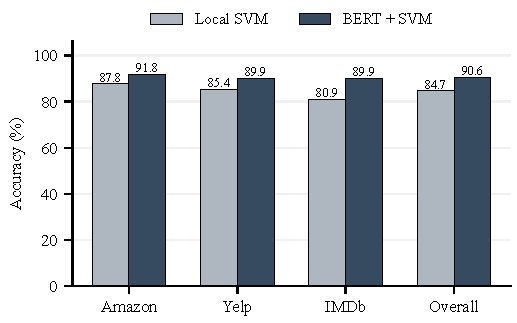
\includegraphics[width=\columnwidth]{benchmark.pdf}
\caption{Accuracy on the fixed positive/negative development benchmark. The vertical axis starts at zero. This is not an independent target-domain evaluation.}
\label{fig:results}
\end{figure}

No controlled ablation in the current evidence isolates the benefit of each idiom rule, specialist rule, or aspect guard. The comparison supports a measured difference between two implemented pipelines, but cannot establish which individual component caused that difference. Repeated use of the public benchmark also prevents treating the improvement as an unbiased estimate of future performance.

\subsection{Spreadsheet and Domain Checks}
Table~\ref{tab:uploads} reports the current outputs for the supplied spreadsheets and product-review CSV. All 1,349 rows were accepted as usable feedback. The parser selected \texttt{Feedback}, \texttt{Feedback / Comments}, and \texttt{Comments}, respectively. The 500-row and 750-row files contain only 15 and 37 distinct review texts; their duplicate counts are 485 and 713. Thus, successful processing of every row does not represent evaluation on 1,250 independent language examples.

\begin{table}[t]
\caption{Supplied-File Processing Results (Predicted Counts)}
\label{tab:uploads}
\centering\footnotesize
\begin{tabular}{lrrrrr}
\toprule
File & Rows & Pos. & Neu. & Neg. & Review\\\midrule
500-row workbook & 500 & 377 & 39 & 84 & 26\\
750-row workbook & 750 & 496 & 32 & 222 & 84\\
AirTag review CSV & 99 & 87 & 4 & 8 & 35\\\bottomrule
\end{tabular}

\smallskip
\parbox{\columnwidth}{\footnotesize ``Review'' denotes flagged records, which overlap the sentiment columns. These counts are model outputs, not accuracy labels.}
\end{table}

The AirTag file illustrates the need for domain-aware interpretation. A product may be praised for finding missing items, even when the review contains words associated with a problem. Contextual inference improves the treatment of several such constructions, but rhetorical questions and long narratives can still fail. Likewise, packaging mentions can concern unboxing rather than fulfillment quality. The implementation reduces broad keyword matches, yet its aspect rules remain an approximation requiring evidence inspection.

Sentiment percentages use only valid analyzed rows. A review can mention multiple aspects, so summed aspect counts can exceed the number of reviews. Duplicate reviews remain in these totals to preserve the input's frequency distribution. A displayed mean confidence is an average of model scores; it is neither a measured accuracy nor the fraction of satisfied customers.

\section{Limitations and Future Work}
The main validity limitation is evaluation reuse. An independent test should be labeled before further tuning, remain frozen, and include genuinely neutral and mixed opinions from the intended customer domain. Splits should group repeated text and related templates to reduce leakage between development and evaluation. Multiple human annotators and adjudication would make ambiguous sentiment labels more defensible.

The current neutral class is supported partly by generated examples and a three-star mapping. Its performance on real neutral feedback is not established. Similarly, aspect extraction has no complete independently annotated precision/recall benchmark, and topic coherence or recommendation usefulness has not been formally measured. Topic labels and business recommendations should therefore support review rather than replace it.

Input validation is deliberately bounded. The English-text check is a character-based heuristic, not a language-identification model. Header recognition is limited to the first 20 rows and known aliases. Merged cells, complex multi-table workbooks, and nonstandard exports may require manual preparation. Review windowing preserves coverage but averages evidence, which may dilute a small yet important complaint in a long document.

Operationally, inference runs on a local CPU with a bounded cache and synchronized model access. The current Flask development server has not been evaluated for high-concurrency production traffic. Local inference avoids transmission to a model API, but exports can still contain customer information and require appropriate handling. No retention policy, authentication layer, or access-controlled database is implemented.

Future work should prioritize a separate labeled target-domain test, probability calibration on an independent validation set, and controlled ablations of the hybrid policy. A trained aspect extractor could be compared with the current lexical rules. Production deployment would additionally require measured throughput, background processing for larger files, authentication, and explicit data-retention controls. Multilingual support should be validated separately rather than inferred from the underlying checkpoint's name.

\section{Conclusion}
InsightPulse implements an end-to-end English customer-feedback workflow that combines contextual BERT inference, a local TF-IDF/SVM specialist, aspect evidence, topic labels, and an interactive dashboard. Explicit file preview, column mapping, source-row preservation, and uncertainty reporting make batch results easier to inspect. The implemented hybrid achieved 90.57\% on the 594-review development benchmark, while three supplied files and 30 regression tests confirmed important integration behaviors. The project demonstrates a reproducible academic system with measurable development improvements. Its next evaluation priority is independent, human-labeled customer feedback covering neutral sentiment and aspect-level correctness.

\section*{Reproducibility}
The implementation and 30-test regression suite were checked on October 15, 2026. The project provides locked dependencies, training and evaluation scripts, saved metrics, and a notebook. The accompanying source package includes the report's numerical evidence and model revision; no new BERT training is required to reproduce inference.

\begin{thebibliography}{00}
\bibitem{pang} B. Pang, L. Lee, and S. Vaithyanathan, ``Thumbs up? Sentiment classification using machine learning techniques,'' in \emph{Proc. EMNLP}, 2002, pp. 79--86, doi: 10.3115/1118693.1118704.
\bibitem{sklearn} F. Pedregosa \emph{et al.}, ``Scikit-learn: Machine learning in Python,'' \emph{J. Mach. Learn. Res.}, vol. 12, pp. 2825--2830, 2011.
\bibitem{bert} J. Devlin, M.-W. Chang, K. Lee, and K. Toutanova, ``BERT: Pre-training of deep bidirectional transformers for language understanding,'' in \emph{Proc. NAACL-HLT}, 2019, pp. 4171--4186, doi: 10.18653/v1/N19-1423.
\bibitem{nlptown} NLP Town, ``bert-base-multilingual-uncased-sentiment,'' model card. Accessed: Oct. 15, 2026. [Online]. Available: \url{https://huggingface.co/nlptown/bert-base-multilingual-uncased-sentiment}
\bibitem{lda} D. M. Blei, A. Y. Ng, and M. I. Jordan, ``Latent Dirichlet allocation,'' \emph{J. Mach. Learn. Res.}, vol. 3, pp. 993--1022, 2003.
\bibitem{uci} D. Kotzias, ``Sentiment Labelled Sentences,'' UCI Machine Learning Repository, 2015, doi: 10.24432/C57604. Dataset distributed under CC BY 4.0.
\bibitem{xenova} Xenova, ``BERT product-review sentiment: ONNX conversion,'' model repository. Accessed: Oct. 15, 2026. [Online]. Available: \url{https://huggingface.co/Xenova/bert-base-multilingual-uncased-sentiment}
\bibitem{onnx} ONNX Runtime, ``Quantize ONNX models,'' documentation. Accessed: Oct. 15, 2026. [Online]. Available: \url{https://onnxruntime.ai/docs/performance/model-optimizations/quantization.html}
\end{thebibliography}
\end{document}
